%%% Local Variables:
%%% TeX-master: "master"
%%% End:

\chapter{Potentive entailment --- \AR{} and \WR{}}
\label{cha:potent-infer-attr}

\begin{note}[Overview]
  In this chapter focuses on understanding potentive entailment, potentive entailment with respect to (specific) abilities, and how potentive entailment with respect to (specific) abilities is used in the cases of interest.
\end{note}

\begin{note}[Potentive entailment]
  Used `potentive entailment' to capture the entailment from `ability to \emph{V} that \(\phi\)' to `\(\phi\) is the case'.
  Roughly, any entailment with the characteristic that in order for there to be some potential event \(e\), \(\psi\) must be the case.
\end{note}

\begin{note}[The focus point]
  Agent has information that admits of potentive entailment.
  Ability to reason to conclusion.
  Conclusion holds.
  And, premises.

  Begin the chapter with a more detailed account of what this entailment is.

  The focus of this chapter how an agent may use the potentive entailment.
  Sketched two types of reasoning.
  \AR{} and \WR{}.

  \AR{}: the agent obtains support for the conclusion of reasoning on the basis of the support they have for having the attribute of being able to reason to the conclusion.
  Support the agent has for antecedent of entailment flows to the consequent.
  Pairing of ability and conclusion.

  \WR{}: obtain support for the conclusion on the basis of the premises.
  The agent establishes a relation of support on the basis of the information that they have the ability to witness reasoning which would establish a relation of support between premises and conclusion.

  Important points about witnessing.
  \begin{itemize}
  \item The agent hasn't witnessing the reasoning they are able to do.
  \item Support the agent establishes is separate from the information that they are able to do the reasoning.
  \item Relation of support that would be established.
  \end{itemize}

  How to understanding information, and what options the agent has for using the information.

  Potentive entailment, events.

  So, there's always a verb.
  Understanding in terms of verb.
  Important.

  Entailment does not depend on some attribute of the agent.
  Reverse.
  Agent has attribute due to potential event.

  In other words, always possible to rewrite information regarding ability in terms that do not mention ability.
  So, we are not required to take some property of the agent to understand entailment --- property of being able to \dots, however this is understood.
  (If reduce to property that is independent of event, then no clear account of relation of support between premises and conclusion.
  Get premises and get conclusion.)
  Hence, not required to appeal (directly) to property in order to obtain conclusion.

  Doesn't suit English so well, but makes sense.

  Doesn't rule out property.
  Don't get into the ontology of potential events.
  So, may reduce.
  Still, from the perspective of reasoning, not required.
  Entailment follows from potential, and potential may require attribution of ability, but only in so far as the antecedent needs to hold.

  First step to \WR{}.
  Second step is using information to establish distinct support relation.
  Event plays same role as property.
  Route support through entailment.
  Argue that this is not the case.
  Understand potential event as providing information about support relation.

  Summarising, three main points.
  \begin{enumerate}
  \item Entailment understood in terms of potential event.
  \item Support distinct from entailment.
  \item Defer establishing support.
  \end{enumerate}

  This is in conflict with~\ref{denied-claim}.
  Relation of support is between premises and conclusion, etc.

  Structure for main part of the chapter split in to section that serve to establish main points.
  Exception that we provide a more detailed account of \AR{} prior to \WR{}.
  For the moment, organise by theme.
  More to each part than focus.
\end{note}

\begin{note}[Plan for chapter]
  The plan for the main part of the chapter is as follows:
  \begin{itemize}
  \item Potentive entailment.
  \item Support
  \item Two ways in which potentive entailment may be used --- \AR{} and \WR{}.
  \end{itemize}

  These sections are followed by optional sections.
  \begin{itemize}
  \item Differences between \AR{} and \WR{}.
  \item (Possibly) further notes on \WR{}.
  \item More on potentive entailment.
    \begin{itemize}
    \item Relation to ability modals.
    \item Interest in entailment itself.
    \end{itemize}
  \end{itemize}

\end{note}

\begin{note}[First part plan]
  We start with potentive entailment, and the section will serve two purposes.
  First, clarify potentive entailment.
  Why it is that the agent has the option of using information about ability to establish certain things about their situation as things stand.

  To do so, we begin with `canonical form' of potentive entailment, stated in terms of potential events, in contrast to ability attributions made to the agent.
  We then see how ability attribution may be understood with the use of events.
  Roughly, instead of a modal quantifier stating that there is an potential event for which the agent is a part, one states that the agent is such that they perform the verb in the relevant event.

  The important upshot of the proposed understanding of potentive entailment is that entailments do not necessarily follow from some attribute of the agent.
  This will help understand \AR{} and \WR{}.
  For, by working with the `canonical form', we have an understanding where the action in the potential event is at the core of potentive entailment, rather than an attribute of the agent.

  The following sections then build on how the `canonical form' may be understood.

  This will provide the setup for the two ways potentive entailment may be used in scenarios of interest.
  In particular, \WR{}, in which support for conclusion is does not require support for ability/event.
\end{note}

\begin{note}[Second part plan]
  Potentive entailment.
  Simply provides information.
  Distinct from establishing a support relation.

  Two ways in which potentive entailment may be used from understanding different support relations made available by entailment.
  Argue that there is no plausible third option, on the basis of potentive entailment (though this does not rule out independent sources).
\end{note}

\begin{note}[Third part plan]
  Potentive entailment.
  Differences in support.

  Potentive entailment is going to hold independent of support.
  Question whether there is further difference, or whether \AR{} and \WR{} come as a pair.

  So, look for ways to distinguish \AR{} and \WR{} with respect to support.
  Argue that these depend on further commitments that we may remain neutral on.
\end{note}

\begin{note}[Wrapping up]
  So, this chapter concludes with a clear understanding of how potentive entailment relates to main argument.
  Understanding of \WR{} and \AR{}.
\end{note}

\begin{note}[Extras]
  Appendix to the chapter contains further remarks on potentive entailment, as it seems that this isn't something that's been discussed too much.
\end{note}


\section{Potentive entailment}
\label{sec:potentive-entailment}

\subsection{The entailment}
\label{sec:entailment}

\begin{note}[Potentive entailment]
  The canonical form of potentive entailment is:
  \begin{enumerate}
  \item In order for there to be potential for some event \(e\) to be witnessed, \(\psi\) must (already) be the case.
  \end{enumerate}
  Intuitively, there is potential for some event \(e\) to be witnessed if there are preconditions for witnessing that must been met, and the potentive entailment identifies \(\psi\) as some such precondition that has been met.

  Term this `potentive entailment' as consequent of the entailment follows from the `potential' construct of the antecedent.
  
  For example, there is potential for Smith to travel to London in time for tomorrows meeting.
  So, there is an aeroplane set to depart no later than midnight tonight for which Smith may purchase a ticket, and so on.
  
  This is `local' entailment.
  It does not look for necessary conditions for an event.
  For example, private jet.
  Given the way things are, no private jet.

  So, hard to determine whether a potentive entailment holds in general.
  May be some exception.

  For present purposes, there is potential for some event to be witnessed.

  Specially, the events of interest are an agent reasoning from some premises to a conclusion.

  \begin{enumerate}
  \item\label{PE:ability:event} As there to be potential for an event of S proving \(\phi\) to be witnessed, \(\psi\) must (already) be the case.
  \end{enumerate}

  Example.

  Finally, change of focus to the agent rather than the potential event.
  Potential for an event of \dots to be witnessed, rewrites to S has the ability to \dots

  \begin{enumerate}
  \item\label{PE:ability:agent} S has the (specific) ability to V that \(\phi\), so \(\psi\) must (already) be the case.
  \end{enumerate}

  Remains an instance of potentive entailment.

  Given that~\ref{PE:ability:event} and~\ref{PE:ability:agent} we avoid the need for an understanding of ability.
  Some worries about what it is for there to be a potential event.
  Suitable analysis may depend on ability, or perhaps ability is analysed in terms of potential events.

  In short, while~\ref{PE:ability:agent} is natural, and our preferred statement, \ref{PE:ability:event} is equivalent.
  Therefore, we will understand the use of potentive entailments involving ability in terms of potential events, rather than on the basis of any particular understanding of ability.

  What matters is the event, and what must be the case in order for the event to be witnessed.

  Important thing to stress is that consequent does not necessarily follow from agent possessing ability.

  Still some differences, deal with these after examples.
\end{note}

\begin{note}[Examples]
  Simple instances of the potentive entailment involve factive verbs, in which the relevant fact holds independently of whether the verb is witnessed.
  \begin{itemize}
  \item Sam has the ability to show that \(19\) is a prime number.
  \item Taylor has the ability to derive Transposition.
  \item Jesse has the ability to \dots
  \end{itemize}

  Note also that the verb does not need to involve some reasoning.
  \begin{itemize}
  \item Corey has the ability to see there is a zebra in the pen.
  \item X has the ability to hear that there is a waterfall nearby.
  \end{itemize}
\end{note}

\begin{note}[Breaking things down]
  An instance of potentive entailment has an antecedent and consequent.
  As may be seen from the examples provided, there are no particular constraints on the consequent of a potentive entailment.
  The antecedent of potentive entailments of interest, however, have two main components:
  \begin{itemize}
  \item\label{pe:part:event} An event.
  \item\label{pe:part:modal} A `potentive' modal applied to the event
  \end{itemize}
  The event in turn has three important components:
  \begin{enumerate}
  \item\label{pe:part:agent} An agent.
  \item\label{pe:part:verb} A verb describing some action performed by the agent.
  \item\label{pe:part:result} Some result of a successful performance of the action described by the verb.
  \end{enumerate}

  Gave a gloss of potentive entailment.

  Key observation 1.
  Possible consequents are determined by the event, rather than the modal.
  Obtain consequent because of the modal.

  So, each of the examples, we obtain the same entailment on the assumption that the event described has happened.

  Contrast.
  Potential for \(e_{1}\) and potential for \(e_{2}\), so potential for \(e_{3}\).
  E.g.\ conjunction introduction.

  In other words, the consequent does not hold because the event is a \emph{potential} event.
  Or, that this is `epistemic'.

  Well, consequent because the event of the antecedent requires the consequent.

  So, that the potential provides a way to get the consequent prior to the event happening.
  No instance of potentive entailment where the consequent follows because the event is potential.
  This is not to deny that there are cases in which entailment relies on potential.

  So, here explaining why the work is done primarily by the verb.
  Might think that using `discovers' is a counterexample.
  Only possible because the action involved is for the moment potential.
  However, the verb itself does the work here.
  Get the consequent that the agent hasn't done the reasoning, but understanding this as simply shifting temporal index.

  So, the important of this key observation is that we further reduce interest in ability.
  We've seen that alternative modal may be used.
  And now that the modal is of secondary importance.

  So, property is seen as surface level.

  Two candidates for the antecedent.
\begin{quote}
  \begin{enumerate}
  \item There is a potential event in which \emph{S} \emph{V}s that \(\phi\).
  \item \emph{S} has the ability to \emph{V} that \(\phi\).
  \end{enumerate}
  \end{quote}
\end{note}

\begin{note}[Still, ability]
  The claim here is that the two are roughly equivalent in the context of the entailments of interest.
  This does not require a general equivalence.

  \textcite{Werner:2011tp} suggests that there's a hierarchy.
  Potentive entailment applies to opportunities.
  So, potential entails ability, but need not be the case that ability requires opportunity.

  However, because we're talking about an application of ability, things are different.
\end{note}


\begin{note}[Two important instances of potentive inference]
  Restate information.
  Apply potentive inference.

  Two important instances of potentive inference
  \begin{enumerate}
  \item Conclusion is the case.
  \item Support for premises.
  \end{enumerate}
\end{note}

\begin{note}[Some variance]
  We get premises and conclusion.

  Here, the important thing is that if the agent doesn't already have the basics, then something further would need to be the case for there to be a potential event.

  Admittedly, there is no clear line.
  For, there are ways to expand the event.

  Example, lighting a match.
  Have match and matchbox in hand.
  Have matchbox.
  Matchbox is in a draw.
  Etc.

  Resolved by placing constraints on the event.
\end{note}

\subsubsection{Obtaining potentive entailments}
\label{sec:obta-potent-enta}

\begin{note}[Quick sketch]
  This is an optional section.
  We explained potentive entailment and given examples.

  Reader may wish for a technical account.
  In this section we sketch one such account.

  We do not argue that the account is wholly adequate.
  However, functional at first pass.

  Two things to do.
  \begin{enumerate}
  \item Establish some equivalence between potential and ability.
  \item Given an account of the potentive entailment.
  \end{enumerate}

  Start by taking a simple possibility understanding of the modal and show how potential and ability fit.
  We will then build on the possibility understanding to fix potentive entailment.
\end{note}

\subsubsection{Modal}
\label{sec:modal}

\begin{note}[Potentive]
  The potentive is straightforward to analyse.

  Fairly clear understanding of event semantics.

  Here, existential quantification over events is replaced by a modal.

  This requires some non-standard existential, but we're not too interested in providing an analysis suitable for semantics.
\end{note}

\begin{note}[Ability]
  Our understanding of ability is basically the same as potentive.

  Ability functions as an equivalent quantifier.
\end{note}

\begin{note}[Avoid ability?]
  A simple corollary of the above observations potentive entailment does not require ability.

  If it is possible to provide information about potential event of reasoning without attributing ability, then we don't need to speak of ability at all, perhaps with the exception of generating intuitive scenarios.

  May wonder how important ability is.

  Difficult case.
  Go for externalism, and co-reference.
  State a conclusion, but the agent would not reason to the conclusion under that description.

  There's a potential event, but it isn't clear that the agent has the ability.

  Doubt this is possible, as agent needs to do something.
  And, ability this seems sufficient for an ability statement.
  So, continue to work with ability.
\end{note}

\begin{note}[Some formal stuff]
  \[(\text{Able}(s,e) \land (V(e) \land \text{agent} = s \land \text{result}(e) = \phi))\]
  There is some event \(e\), such that \emph{s} is able to bring about, and \(e\) consists of \emph{s} \emph{V}ing with the result that \(\phi\).

  The quantification here is somewhat familiar to Lewis' counterpart theory.

  Understand ability as relating the agent directly to an event.
  Alternative it to take a truth value.
  \((\text{Able}(s,\exists (V(e) \land \text{agent} = s \land \text{result}(e) = \phi))\).

  Close to having a possible world with \(\phi\) and accessibility relation.
  Interpret the non-standard existential in this way, if it helps.
  There is some possible world and some event in that world, such that the agent at the world of evaluation is able to perform the event witnessed at the possible world.

  In both cases, it's the role of the event.

  \begin{figure}[h]
    \begin{subfigure}{.5\textwidth}
      \centering
      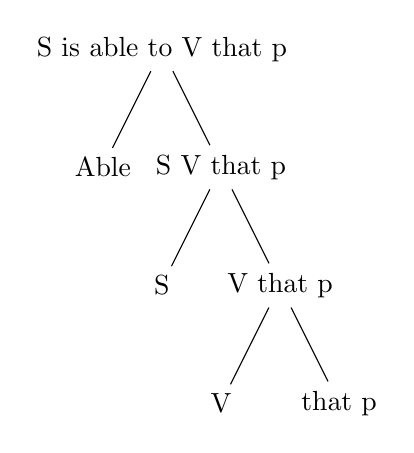
\begin{tikzpicture}[
        ]
        \node{S is able to V that p}
        child {node {Able}}
        child {node {S V that p}
          child {node {S}}
          child {node {V that p}
            child {node {V}
            }
            child {node {that p}
            }
          }
        };
      \end{tikzpicture}
    \end{subfigure}
    %
    \begin{subfigure}{.5\textwidth}
      \centering
      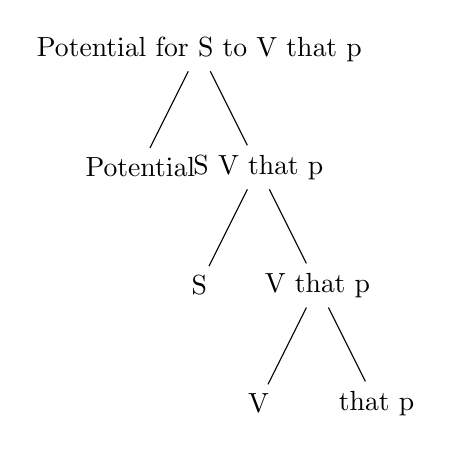
\begin{tikzpicture}[
        ]
        \node{Potential for S to V that p}
        child {node {Potential}}
        child {node {S V that p}
          child {node {S}}
          child {node {V that p}
            child {node {V}
            }
            child {node {that p}
            }
          }
        };
      \end{tikzpicture}
    \end{subfigure}
  \end{figure}
  Suggestion here is that there's really nothing too interesting.
  In both cases it seems possible to have a complete description of the witnessing event prior to the introduction of a modal.
  Only complexity involved is projecting agent from event in order to apply ability.
\end{note}

\subsubsection{Entailment}
\label{sec:entailment-1}

\begin{note}[Understanding potentive entailment]
  The key parts of the entailment are the relation between ability and the verb.

  Certain things must be true in order for the verb.
  These are the things which are obtained by the potentive entailment.

  In the case of reasoning, note that there must be premises from which the agent works from.
\end{note}

\begin{note}[The entailment]
  Take some arbitrary witnessing event.
  If \(\psi\) follows from the (arbitrary) witnessing event, then we have an instance of the potentive entailment.

  Pretty much the same as reasoning with existentials.
\end{note}

\begin{note}[Expanding the event]
  The description of the witnessing event given is minimal.
  Still, simply add in more detail as desired.
\end{note}


\begin{note}[Counterfactual]
  One option is counterfactual.
  This is true, and then consider all of those things some that if they we're true, potential wouldn't be true.
  Consider change to the actual world that would result from false consequent, and figure out whether potential still holds.

  Problem here is that counterfactuals are tricky.

  Minimal change may still result in potential.
  Chess example, if strategy doesn't exist, then it's not clear how to understand this.
  Some other rules of chess, and strategy may still exist.
\end{note}

\begin{note}[More direct]
  Preferred option is to consider all witnessing events.
  No matter how things turn out, the truth of \(\phi\) persists throughout event.

  What about changes?
  So, there's some potential event, because of some change to the rules of chess.
  Hence, there is a possible event, but relies on an unexpected development.
  Problem with potential?
  Arguably same issue holds for ability.

  However, it's then going to be the case that there is some change.
  Problem here when it comes to reasons, as the agent doesn't have the reasons available.

  Observation here is that \(\phi\) is an enabling condition.
  Potential just in case that it does not depend on further enabling conditions that are not yet the case.


  So, suggestion that if something holds throughout every event, then it holds of the actual world.
  Basically, this rules out an enabling condition that is not true.

  Hence, \(\phi\) is an enabling condition, and does not require additional enabling conditions.
\end{note}

\begin{note}[Still issue of underspecified event]
  Returning to the matchbox.
  Different preconditions.
  Well, depends on how the event is understood.

  Use this idea to suggest some troubles.
  By, extending events to include establishing what seem to be preconditions.
  Suggest that this is taken care of by understanding of event.
\end{note}

\subsubsection{Summary of details}
\label{sec:summary-details}

\begin{note}[Seen]
  Suggested that potential and ability may be treated the same.
  Both considered as a `refined' modal with existential force.

  Narrowed the modal to show how potentive entailment follows.

  No significant insights.
  Defence of some claims that rested on intuition in previous section.
\end{note}


\subsection{Our interest in potentive entailment}
\label{sec:our-inter-potent}

\begin{note}[Two important instances of potentive inference, recap]
  Restate information.
  Apply potentive inference.

  Two important instances of potentive inference
  \begin{enumerate}
  \item Conclusion.
  \item Premises.
  \end{enumerate}
  Potentive entailment ensures that these are the case, among other things.
  Key is that all that remains is the agent reasoning from the premises to the conclusion.
\end{note}

\begin{note}[Reasoning and premises]
  Important to note is that in cases of reasoning, the potentive entailment may be applied to obtain the availability of premises.

  The difference is the role of these premises.
\end{note}

\begin{note}[Restriction on instances of potentive entailment]
  We're interested in certain examples as the agent has all of the resources required, so to speak.

  May resist account of potentive entailment, as it seems the entailment applies more generally.
  For example, same principle applies when it's possible for the agent to acquire some information.

  Events are flexible.
  

  To illustrate, place the reasoning examples behind a conditional.
  \begin{itemize}
  \item If you teach Sam \dots [factoring method], then Sam will have the ability to show that \(19\) is a prime number.
  \end{itemize}
  Intuitively, this is the result of assuming that some additional property holds of the agent.
  Hence, \(\alpha(s) \rightarrow \dots\).
  For, \(\alpha(s)\) will allow the attribution of ability to be true.
\end{note}

\section{\AR{} and \WR{}}
\label{sec:ar-wr}

\begin{note}[Overview]
  Interest is in how potentive entailment is used.

  A clearer understanding of \AR{} and \WR{}.

  The significant difference is with reasoning.
  \AR{} uses (a variation of) the potentive entailment to obtain support/traces a support relation through potentive entailment.
  \WR{} uses information obtained by the potentive entailment to obtain support.
\end{note}

\begin{note}[So far]
  Potentive entailment.
  Focus on the event.

  Alternative to surface reading.
  No necessarily by virtue of some stronger understanding of ability.

  Important for how information about (specific) ability is used.

  Precondition for potential event.

  So, that the agent has the ability (or that the event is potential) does the job.
  Or, that there is a relation of support between preconditions for the potential event.
\end{note}

\begin{note}[Structure]
  Two premises.
  \begin{enumerate}
  \item Support doesn't necessarily follow entailment.
  \item Clarify the two different types/conceptually possible.
  \end{enumerate}
  The section then concludes with a handful of additional observations regarding \AR{} and \WR{}.
\end{note}

\subsection{Entailment and support}
\label{sec:entailment-support}

\begin{note}[Overview]
  The previous section provided an overview of potentive entailment.
  The following sections will explore the use of potentive entailment when an agent reasons with information that they have the ability to reason to some conclusion.
  The present section argues a premise that will be used in the following sections.

  \begin{enumerate}
  \item\label{PE+S:epistemic} Entailment is `epistemic'
  \item\label{PE+S:diff-support} Instances in which information about an entailment allows an agent to establish a relation of support between some premise and conclusion, where the premise and conclusion may be distinct from the antecedent and consequence of the entailment.
  \end{enumerate}
  The upshot of~\ref{PE+S:diff-support} is that it is, at least conceptually, possible that any agent may recognise that a potentive entailment holds, and uses the entailment to establish support.
\end{note}

\begin{note}[Epistemic]
  The entailment is epistemic.
  Meaning, information of antecedent is sufficient to establish consequent.
  It is not the case that the consequent holds because the antecedent holds.
\end{note}



\begin{note}[Quick test]
  Potential \(e\) is the reason why \(\psi\).
  \(\psi\) is the reason why there is potential \(e\).

  Some good instances and some bad.

  Bad is the flight example.
  These are, in the appropriate sense, preconditions.
  So, the relation of support is inverted.

  However, from epistemic perspective, things may go the other way.
\end{note}

\begin{note}[Tracks example]
  There are tracks \dots

  So, why provides support?

  Another is reading a clock.
\end{note}

\begin{note}[Translation]
  Someone says something false.
  Hold them to be a liar.

  Translation.
  A little murky.

  Still, develop a little more.
  Informer provides basics of translation.
  Now the agent has translated.
\end{note}

\begin{note}
  These are examples in which it seems, at least on the surface, plausible that information provided allows the agent to establish a support relation.
\end{note}

\begin{note}[Two premises so far]
  \begin{enumerate}
  \item Potentive entailment need not establish support.
  \item Instances in which information allows for distinct support relations.
  \end{enumerate}
\end{note}

\begin{note}[Okay with uRa]
  As an aside, these examples are compatible with \ref{denied-claim}.
  The issue is with what establishes support.
  \ref{denied-claim} only details `access', and in these examples the options for support seem accessible.
\end{note}

\subsection{Entailment, support, and the ability to reason}
\label{sec:enta-supp-abil}

\begin{note}[Ability to reason]
  The important thing to keep in mind is that if the agent has the ability, then the agent has propositional support, so to speak.
  This is not required for potentive entailment, which is far more general.
  However, we develop \AR{} and (in particular) \WR{} with this assumption in mind.
\end{note}

\begin{note}[\AR{} and \WR{}]
  Have conclusion obtained by potentive entailment.

  Support is traced from ability/potential.
  Support is traced from premise obtained by potentive entailment.
\end{note}

\begin{note}[Diagram]
  \begin{figure}[h]
  \begin{subfigure}{.5\textwidth}
    \centering
    \begin{tikzpicture}[
      ->,
      >=stealth',
      % auto,
      node distance=0cm, every text node part/.style={align=center},
      ]

      \node [] (c) at (0,0) {};
      \node [] (d) at (-3,0) {};
      \node [] (e) at (3,0) {};
      \node [] (f) at (0,-2.1) {};

      \node (1) at (0,-.1) {Ability};
      \node (2) at (0,-2) {Conclusion};

      \draw [->] (1.270) to [] node[left] {} (2.90);
    \end{tikzpicture}
    \caption{\AR{}}
    \label{fig:AR:support}
  \end{subfigure}
  % \hfill
  \begin{subfigure}{.5\textwidth}
    \centering
    \begin{tikzpicture}[
      ->,
      >=stealth',
  % auto,
      node distance=0cm, every text node part/.style={align=center},
      ]

      \node [] (c) at (0,0) {};
      \node [] (d) at (-3,0) {};
      \node [] (e) at (3,0) {};
      \node [] (f) at (0,-2.1) {};

      \node (premise) at (0,-.1) {Premise};
      \node (conclusion) at (0,-2) {Conclusion};

      \node (x) at (-2,-1.05) {Ability};
      \draw [->] (1.270) to node[left] (3) {} (2.90);

      \node (4) [left of=3, xshift=-2cm] {}; % {\(\exists f (f\Phi = \psi)\)};
      \draw [-{Circle[open]}, dashed] (x.0) to (premise);
      \draw [-{Circle[open]}, dashed] (x.0) to (conclusion);

    \end{tikzpicture}
    \caption{\WR{}}
    \label{fig:WR:support}
  \end{subfigure}
  \caption{Relations of support for \AR{} and \WR{}}
  \label{fig:ARandWR:support}
\end{figure}
\end{note}

\begin{note}[Examples of support relation]
  The interesting issue is the inaccessibility of the premises.
  However, there are other examples in which the same structure is present, but premises are accessible.
  
  Are there other instances of information being used in this way?

  Plausible that go from appearance to support.

  `You are looking at a dog'.

  Here, the agent can infer from testimony that the animal is a dog.
  On the other hand, the agent can take the information to establish a support relation.
  So, visual perception support that the animal is a dog.

  Or, a little better.
  These are coyote tracks.
  Then, different ways to support presence of coyote.
  One is the information provided.
  The other is the tracks.
\end{note}

\begin{note}[The event]
  Two ways for the potentive entailment to function.
  Both \AR{} and \WR{} focus on the witnessing event.

  \emph{V}ing that \(\phi\).
  \begin{itemize}
  \item \(\phi\) must be the case in order for the agent to \emph{V} that \(\phi\).
  \item In order for the agent to have the attribute \dots
  \item \(\phi\) is the result of the agent \emph{V}ing.
  \item As a result of witnessing the ability \dots
  \end{itemize}

  So, \AR{} doesn't consider the relevant witnessing, only what must be the case in order for there to be a witnessing event.
  By contrast, \WR{} focuses on guarantees about what transpires in the witnessing event.
\end{note}

\begin{note}[Multiple support relations]
  \AR{} and \WR{} differ in terms of support relations.
  This is the most important distinction for the broad argument of the thesis.

  Focus is on particular kind of ability: general to specific.

  Still, this provides us with at least three distinct support relations that may follow from an agent receiving information that they have the ability to reason to some conclusion, and prior to witnessing the ability.
  \begin{enumerate}
  \item \AR{}
  \item \WR{}
  \item Precondition of receiving information.
  \end{enumerate}
  In simple cases, all three may be available to an agent after receiving information.

  Question about how these interact.
  Support does not seem additive.
  
\end{note}

\subsection{\AR{}}
\label{sec:ar}

\begin{note}[The way to phrase this]
  Well, at some point the agent is in a position to attribute sufficient support to themselves.
  Start with the easiest case, ability, and then expand to other cases.
\end{note}

\begin{note}[Attribution]
  \AR{} establishes a relation of support between an agent's (specific) ability to reason to some conclusion, and some proposition which follows via potentive entailment.
  Take the information, and link.

  We have argued that potentive entailment is understood via preconditions for witnessing events of the ability.
  However, as the agent performs the action described by the verb, it makes sense to attribute the agent the property of being able, or in a position, to bring about the potential event.

  Properties are cheap.
  On my desk is a cup of coffee.
  The cup has the property of containing coffee.
  The coffee has the property of being in the cup.
  I have the property of having poured the coffee into the mug.
  Previous moments have the property of being moments for which I was pouring coffee in to the cup.
  And, I have the property of being in a position to drink the coffee in the cup.

  For sure, it's something that has not happened, but so long as there is sense to be made of a potential event, there's a corresponding property.

  Might reduce why this is true to something else, particular path of mental steps.
  But we're still going to have a property of this kind.

  Though potentive entailment is understood in terms of events, the property of being able to reason to some conclusion references some potential event and we may chain together a derived instance of potentive entailment.
  \begin{enumerate}
  \item As the agent has the (specific) ability, there is a potential event,
  \item potential event only if \(\phi\) is a precondition of the potential event, therefore
  \item Agent has (specific) ability, \(\phi\) holds.
  \end{enumerate}
  As we are interested in the support appealed to by the agent, and not {\color{red} some kind of metaphysical} support relation, the derived instance of potentive entailment provides a route for the agent to transmit support they have for having the ability to the relevant precondition for the potential event.

  In short, it seems that derived potentive entailment is suitable for transmitting support.
  Whatever support the agent has for the (specific) ability also provides support for the preconditions for witnessing the (specific) ability.

  

  Countless examples.
\end{note}

\begin{note}[Ability is not strictly required for attribution]
  Described \AR{} with ability.
  Have seen that this can be reformulated in terms of potential event.
  The same pattern holds with potential event.

  For example, support for potential event, so conclusion holds.
\end{note}

\begin{note}[Premises exist?]
  Here, may wonder whether existence of premises is doing the work?
  Suggestion is that support from premises, but unaware of what support that is.
  It seems the agent obtains support for existence.

  For example.
  Information that shape consists of three lines.
  Recall tracking example.
  These are coyote tracks.
  Exist coyotes nearby.
  Area is dangerous.

  Don't need to say that the area is dangerous because of the specific coyotes nearby.
  The existential is sufficient.
\end{note}

\begin{note}[No to existential]
  If existential, then a potential event variant of attribution.
  This is an additional step.
  Instead of going straight to conclusion, this is drawing out additional features.
\end{note}

\begin{note}[Example, fire]
  Alarm is ringing, so there is a fire.

  Same basic idea.
\end{note}

\begin{note}[Relation to uRa]
  There is no immediate relation between \AR{} and~\ref{denied-claim}.

  \ref{denied-claim} talks about access to premises.
  \AR{} states that there is a support relation.

  \ref{denied-claim} enters the picture when observing that the agent has information about ability prior to witnessing ability.

  If the agent has information about (specific) ability and the agent has support for information, then extending support from ability to result is consistent with~\ref{denied-claim} as the only required premise is that the agent has the ability.
\end{note}

\begin{note}[Requires support for ability]
  Before turning away from \AR{}, let us stress that \AR{} requires the agent to have support for the (specific) ability in order to obtain support for the conclusion.
  Hence, if the agent does not have support for the (specific) ability, then they will not have the option of obtaining support for the conclusion via \AR{}.
\end{note}

\subsection{\WR{}}
\label{sec:wr}

\begin{note}[Overview]
  In section~\ref{sec:ar-wr} we outlined the key distinction between \AR{} and \WR{} for the purpose of the overarching argument of this thesis.

  Understanding \WR{}.
\end{note}

\begin{note}[Work backwards for the event]
  Work backwards for the event.

  The potential event involves the agent reasoning to some conclusion.
  Reasons from premises.

  As event of reasoning is potential, preconditions are satisfied.
  Hence, conclusion holds, and premises sufficient for conclusion in line with \ref{prem:bP}.
\end{note}

\subsubsection{First pass: Pre-existing propositional support}
\label{sec:first-pass:-prop}

\begin{note}[Outline]
  Our first pass at a detailed understanding of \WR{} assumes that the premises provide the agent with propositional support for the conclusion, independent of whether the agent has, or will, do the reasoning.

  On a standard picture, the agent obtains doxastic support from propositional support if attitude toward conclusion is appropriately connected to propositional support.
  For the agent to obtain doxastic support, need appropriate connexion, not additional support.

  Hence, this suggests that what's missing is the appropriate connexion.

  That is, two components.
  \begin{enumerate}
  \item Support
  \item How the agent uses this support to get conclusion.
  \end{enumerate}

  As the agent already has sufficient support for the conclusion on basis of premises, our task is to explain how information about ability/potential event allows the agent to appropriately connect attitude toward conclusion to premises.

  Start with propositional and doxastic.
  Then work out second point.
\end{note}

\begin{note}[Propositional and doxastic support]
    Our use of support falls closer in line with doxastic justification as opposed to propositional justification.
  Roughly, following \textcite{Silva:2020aa}:

  \begin{quote}
    Propositional Justification (PJ): S has propositional justification to believe that p iff S has sufficient epistemic reasons to believe that p.

    Doxastic Justification (DJ): S has a doxastically justified belief in p iff
    \begin{enumerate*}[label=(\roman*)]
    \item S has propositional justification to believe that p,
    \item S believes that p, and
    \item S's belief in p is appropriately connected to S's sufficient epistemic reasons to believe p.
    \end{enumerate*}
  \end{quote}

  These are fairly neutral definitions.

  \ref{prem:bP} informs our understanding of sufficient epistemic reasons.
  However, no full account.

  Important for our purposes, however, is that although sufficient epistemic reasons is undefined, it is implicit that these do not reduce to the agent having doxastic support for p.
  For, propositional support is part of the definition of doxastic support.
  Hence, if sufficient epistemic reasons to believe p were defined in terms of having doxastic support, then this would lead to circularity.

  This is the important property.
  For, in the cases of interest the only thing the agent lacks prior to information is the second two conditions for doxastic support.
  Hence, so long as these characterisations are adequate, the agent will have propositional support.
  For, it seems there is nothing else that could be added.
\end{note}


\begin{note}[Illustration]
  \begin{figure}
    \begin{subfigure}[h]{.5\linewidth}
      \centering
      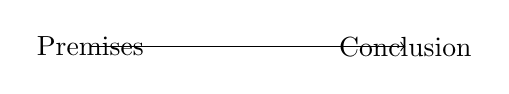
\begin{tikzpicture}[scale=.5]
      \node at (0,0) {Premises};
      \node at (8,0) {Conclusion};
      \draw[->] (0,0) -- (8,0);
    \end{tikzpicture}
    \caption{Propositional}
    \end{subfigure}
    \begin{subfigure}[h]{.5\linewidth}
      \centering
      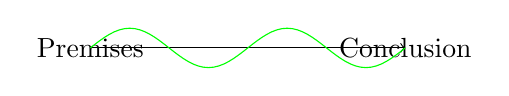
\begin{tikzpicture}[scale=.5]
      \node at (0,0) {Premises};
      \node at (8,0) {Conclusion};
      \draw[->] (0,0) -- (8,0);
      \draw[green] (0,0) sin (1,.5) cos (2,0) sin (3,-.5) cos (4,0) sin (5,.5) cos (6,0) sin (7,-.5) cos (8,0);
    \end{tikzpicture}
    \caption{Propositional and doxastic}
    \end{subfigure}
  \end{figure}
\end{note}

\begin{note}[Future]
  Suggestion is to introduce idea of a \future{}.

  Understanding of doxastic support is appropriate connexion.
  Information about ability means that appropriate connexion may be established.
  A \future{} stands in place of the relation, it fixes that the attitude is connected to premises, etc.
  So, whatever the appropriate connexion would be, any resolution of the \future{} will satisfy that connexion, and the information about ability (in part) allows the agent to be confident that they may fulfil the \future{}.
\end{note}

\begin{note}
    \begin{figure}
    \centering
    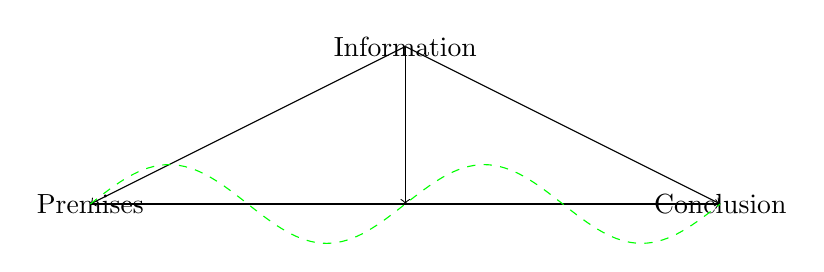
\begin{tikzpicture}
      \def\iHeight{2}
      \node at (4,\iHeight) {Information};
      \node at (0,0) {Premises};
      \node at (8,0) {Conclusion};
      \draw[->] (0,0) -- (8,0);
      \draw[->] (4,\iHeight) -- (8,0);
      \draw[->] (4,\iHeight) -- (0,0);
      \draw[->] (4,\iHeight) -- (4,0);
      \draw[green, dashed] (0,0) sin (1,.5) cos (2,0) sin (3,-.5) cos (4,0) sin (5,.5) cos (6,0) sin (7,-.5) cos (8,0);
    \end{tikzpicture}
    \caption{Sketch}
  \end{figure}
\end{note}

\begin{note}[Expand tracking example]
  Consider tracking example.
  Here, on the relevant interpretation, the information provided to the novice allowed the novice to establish support relation.
  Understood here as providing information about to establish an appropriate connexion.
  And, given this information the novice goes ahead and establishes the (appropriate) connexion.

  Vary the example a little.
  Suppose the novice is provided with a book containing the information provided by the informer.
  Given understanding of base case, understand that the book is going to detail how to establish an appropriate connexion.
  Then, the novice reads the book, and fills in the detail.

  After reading the book, agent has doxastic support.

  Before reading the book, a more complex attitude.
  Conclusion on the basis of propositional support the novice has, and the result of establishing an (appropriate) connexion via the relevant contents of the book.
\end{note}

\begin{note}[New example]
  Consider an abbreviated proof.
  Look at the premises and conclusion.
  So, have propositional support.
  Quite tired, so fail to see how the conclusion is obtained from premises.

  On the one hand, this has been reviewed, etc.\ so route to doxastic support.
  However, given understanding of material, then after some sleep and a cup of coffee, you'll recreate the reasoning in detail.

  Hence, hold the conclusion on the basis of premises, with a \future{} representing the appropriate connexion to be filled in.

  
\end{note}

\begin{note}[Does not depend on application]
  The idea here is fairly general.
  Our interest is in support.
  However, it is more general.

  Simply tracing out something to be filled when required.
\end{note}

\begin{note}[Intuition, logic example]
  Final example by an analogy.

  Consider rules for existential.
  Take a fresh variable.
  Standard is to complete the proof by discharging the assumption.

  Instead, update the assignment function.

  So, three objects, some conditionals.
  Introduces some names.
  Not sure what the name refers to.
  Some property will be revealed, and interpretation fixed.
  
  Perhaps useful to think about in terms of existential reasoning.
  Here, however, we don't discharge the fresh variable.
  Rather, it hangs around in wait for fixed a reference via an updated assignment function.
\end{note}

\begin{note}[Deferring]
  So, \future{} is result of deferring establishing what the connexion is.
  At the time, the agent simply establishes the connexion on the basis of the information they have.
\end{note}

\begin{note}[Existential]
  Support is flowing from the premises to the conclusion.
  It is not from ability.

  Difference is clearest when considering the instance of \AR{} in which the agent appealed to the attribute of having propositional support for the conclusion.
  In the case of \AR{} the agent did not appeal to the propositional support.
  Rather, the agent appealed to having propositional support.

  Contrast, \WR{} takes the propositional support that satisfies the existential.
\end{note}

\begin{note}[Contrast with \ref{denied-claim}]
  Noted that \ref{denied-claim} is understood with respect to doxastic, and here's where the incompatibility comes in.
  For, \ref{denied-claim} holds that a \future{} is no good.
\end{note}

\begin{note}[Asynchronous]
  Asynchronous, as reasoning is deferred.
  Some difficulty.
  However, `weak' asynchronous, as the support `exists', so to speak.
\end{note}

\begin{note}[Key difference]
  The key difference between \AR{} and \WR{} is that with \WR{} the agent does not rely on ability/potential event for support.
  Rather, the agent relies on the support that they have for the premises which is independent of the ability information.

  Information in \WR{} does not support conclusion.
\end{note}

\subsubsection{Difficulty with first pass}
\label{sec:diff-with-first}

\begin{note}[Overview]
  The first pass assumed something about propositional support.
  That there is propositional support whether or not the agent does the reasoning.

  Whether or not agree with assumption, consider a pair of contrasting accounts of propositional support, and see how this assumption is important.

  After so doing, consider whether we can avoid assumption made.
\end{note}

\begin{note}[Different view of propositional]
  For example, \citeauthor{Turri:2010aa} argues for~\ref{Turri:PJ}.
  \begin{quote}
    \begin{enumerate}[label=(\textbf{PJ}), ref=(\textbf{PJ})]
    \item\label{Turri:PJ} Necessarily, for all \emph{S}, \emph{p}, and \emph{t}, if \emph{p} is propositionally justified for \emph{S} at \emph{t}, then p\emph{} is propositionally justified for \emph{S} at \emph{t} \textsc{because} \emph{S} currently possesses at least one means of coming to believe \emph{p} such that, were \emph{S} to believe \emph{p} in one of those ways, \emph{S}'s belief would thereby be doxastically justified.
    \end{enumerate}
  \end{quote}
  If so, then the availability of propositional support is secured by the potential event of reasoning.
  Hence, it seems that this reduces to a case of \AR{}.
  For, if the agent does not appeal to support for witnessing event, then the agent does not have grounds for holding that they have support for conclusion.
  It is not sufficient to observe that the agent has support so long as information about potential holds.
  Instead, the potential is doing the work in providing the agent with propositional support.

  Of course, \citeauthor{Turri:2010aa} doesn't require that the agent be aware.
  But this doesn't solve the problem.
  The issue is that the two instances of support coincide.

  It's somewhat straightforward to recast (\emph{PJ}) as `because the agent has the ability'.
  Indeed, \citeauthor{Turri:2010aa} speculates that propositional support is governed by abilities.
  Though, the exact relation between \citeauthor{Turri:2010aa}'s constraints and are use of ability is unclear.
  At the very least, \citeauthor{Turri:2010aa}'s seems weaker, as we require a sufficient collection of preconditions to be satisfied.
\end{note}

\begin{note}[Note]
  The difficulty is that if \citeauthor{Turri:2010aa} is followed, then there's no support to do the work.
  This does not mean that the premises are unavailable.
  Instead, the premises are inert.
\end{note}

\begin{note}[Same from \citeauthor{Goldman:1979ui}]
  \citeauthor{Goldman:1979ui} offers \emph{ex ante} justification.
  \begin{quote}
    Person \emph{S} is \emph{ex ante} justified in believing \emph{p} at \emph{t} if and only if there is a reliable beliefforming operation available to S which is such that if \emph{S} applied that operation to his total cognitive state at \emph{t}, \emph{S} would believe \emph{p} at \emph{t}-plus-delta (for a suitably small delta) and that belief would be \emph{ex post} justified.\nolinebreak
    \mbox{}\hfill\mbox{(\citeauthor[21]{Goldman:1979ui})}
  \end{quote}
  Note that \citeauthor{Goldman:1979ui} talks of the `total cognitive state' of the agent at \emph{t}-plus-delta.
  It seems clear that the cognitive state of the agent at \emph{t} is relevant on in so far as the delta in \emph{t}-plus-delta is suitably small.
\end{note}

\begin{note}[Example?]
  However, following present line of thought, propositional support is a derived relation.
  It is a relation derived from some `attribute'.

  Clearest to see by recalling reasoning above.
  Project from event.
\end{note}

\begin{note}[Basic point]
  The observation here is that these accounts may taken as trouble for \WR{}, and in turn as partial support for \AR{}.
  Partial support for \AR{} as these accounts of propositional support are of propositional rather than doxastic support, and \AR{} is concerned with doxastic support.
  So, need to be furnished to show that an agent has the option of obtaining support for the conclusion of the reasoning that they are able to perform.

  It seems rather that this is an objection to the basic idea of \WR{}.
\end{note}

\begin{note}[This is trouble from \WR{}/Something about evidential relations]
  Not that these come easy.

  Basic understanding of propositional support.
  Seems support is a relation between premises and conclusion, or base and proposition.

  Common to talk in terms of `\emph{p} is propositional justified for \emph{S}'.
  Here, though, expanded.
  Sufficient reasons to believe that \emph{p}, and \emph{S} has those reasons.

  And, \textcite{Silva:2020aa} highlights troubles with evidential relations, and epistemic reasons.

  Similarly, because \emph{S} has ability, \emph{S} ought not to hold that \dots
\end{note}

\begin{note}[Bracketing possible issue]
  A possible lesson to be drawn from \citeauthor{Turri:2010aa} and \citeauthor{Goldman:1979ui} is that there is no clear relation of support between premises and conclusion.
  Don't make sense to subdivide the agent's total cognitive state, or separate the means by which the agent may come to believe \emph{p}.

  This is the foundation of a challenge to~\ref{prem:bP}.

  However, this isn't too much of a concern.
  Important for our purposes is preconditions.
  Talk of premises, is intuitive, what we're after, though, is some way of obtaining support which doesn't reduce to \AR{}.
\end{note}

\subsubsection{Second pass: Futures grating support}
\label{sec:second-pass:-futures}

\begin{note}[Is this only surface deep?]
  The problem stems from whether it makes sense to talk of support that the agent may appeal to which is distinct from the agent's ability to witness the reasoning.

  If the premises aren't providing support, then it doesn't seem as though the agent is able to obtain support for the conclusion in a way distinct from \AR{}.

  Tentatively, then, \WR{} requires a particular understanding of propositional support.

  Note, this is only a problem for one part of the first pass.
  Do not have the option of relying on pre-existing support relation.

  That the premises must stand in an existing support relation may be challenged.

  We have already seen that it is plausible that any support obtained prior to witnessing the reasoning is distinct from the support that would be obtain by witnessing the reasoning.

  Suggestion is that support flows through future relation.
\end{note}

\begin{note}[Support]
  Well, the point here is that the support relation may be considered with an reference that has not yet been fixed.

  So, instead of taking a `pre-existing' support relation, as in the case of propositional support, we have a support relation which doesn't yet have a referent.
  Finding a reference for the relation is deferred.

  The novelty here is that support transmits through deferred support.
  Intuitively, this is asynchronous.
  The agent establishes relation of support given information.
  Then, at some other times details exactly what the relation of support is.
  The unique thing in these cases is that the agent has information about what the result of the deferred detailing is, and thus has the option of establishing a relation of support to be filled in.
\end{note}

\begin{note}[Intuition]
  At this point, a little intuition would be useful.
  Kind of like a future.
\end{note}



\begin{note}{Future}
  So, this gives us a model of what a future is.

  Talking of functions here, worry about `total cognitive state'.
  Here, that may be the relevant argument.
\end{note}

\begin{note}[The really important thing]
  Support is flowing from the premises to the conclusion.
  It is not from ability.

  If propositional support that does not reduce to ability, then no need to take this as a primitive.
  If not, then perhaps.
\end{note}

\begin{note}[Why does the agent obtain support?]
  Futures are something of a primitive.
  And support is very general.
  So, not really possible to work from some more basic premises.

  Instead, consider it a hybrid of the two types of propositional support considered.
  Like general propositional support, holds whether or not agent has done reasoning.
  Like \citeauthor{Goldman:1979ui} etc.\ potential events inform.

  Not assuming propositional support.
  Or, assuming that information about potential event may not provide information about pre-existing relation of support.
  So, where does support come from?

  Well, we've got a future.
  Associated promise.
  The promise is not providing support.

  What is added is reasoning.

  The potential event, then, ensures that the relation may be filled in.

  Support for conclusion because potential event provides sufficient information to establish relation of support.
  What remains is fixing the specifics of the relation.

  Well, the support for the conclusion just is the support that the agent would obtain from reasoning.
  The thing is that the reasoning part is the only thing that's missing.
  It's the reasoning that is deferred.
  I.e.\ asynchronous.

  Illustration with standard case, then cutting a pasting for a different temporal order.
\end{note}

\begin{note}[Other cases]
  Thinking back to the tracking case may be helpful.
  In the case, information allowed the agent to establish (doxastic) relation of support.

  If propositional support doesn't work as expected, then prior the agent did not have propositional support.
  (This is a plausible reading of \citeauthor{Turri:2010aa}'s remarks on the more fundamental stuff that goes on with support, though could be avoided.)

  The difference is that the information is restricted in the case of interest.
  But the future \emph{functions} in an analogous way.
  It just doesn't carry (sufficient) information about the relation.
\end{note}


\begin{note}[How support works]
  In the case of reasoning, the result will be that the agent has information about premises.
  Here, it is important to note that the agent has `propositional' support for the premises, independent of the ability information.
  So, the agent does not need to appeal to the existence of the event as a premise in obtaining support for the conclusion.
  The only relevant support the agent has is the support for the premises.
\end{note}

\begin{note}[Similar applications of the basic idea]
  Introduce idea that this is something of a placeholder.
  Perhaps use the example from names with an as yet unidentified reference to provide additional motivation.

  The idea is similar in principle.
  There is someone out there in the world.
  Just as there is support that the agent may use.
  So, the remaining task is to fix the interpretation of the name.
  Likewise, the remaining task for the agent is to witness the relation of support.

  In both cases, establishing the additional stuff is useful.
  Foremost, resolves the possibility that the `future' may not be resolved.
  And, other minor benefits in terms of further information.
\end{note}

\begin{note}[Giving up on synchronous support]
  This is something of a cost.
  Cost captured in large part by~\ref{denied-claim}.

  Difficult.
  For, if basic understanding of propositional support, then still require something to explain how the agent transforms this to doxastic support.
  

  Still, two plausible pictures.
  Pre-existing propositional support.
  Support obtained through use of a future.
\end{note}

\begin{note}[Upshot]
  Main upshot is relation of support.

  One nice upshot is that there is a clear link between the support obtained prior to reasoning, and the support obtained by reasoning.
  It's filling in the deferred reasoning.

  May expand.
  For example, with a promise to resolve the support relation.

  Another upshot is that ???
\end{note}


\subsection{Distinction between \AR{} and \WR{}}
\label{sec:dist-betw-ar}

\begin{note}[Overview]
  The important difference is what supports the conclusion.

  Here, we suggest that further differences depend on additional commitments.
\end{note}


\begin{note}[Key Issue]
  The key issue is whether the agent obtains support for all the relevant preconditions of witnessing the ability by witnessing.
  And, whatever follows from this, e.g.\ in terms of commitments and so on.

  If so, then anything that follows from \AR{} also follows from \WR{}.
  Conversely, as the agent does not obtain information about how the ability is witnessed, it seems what follows from \WR{} also follows from \AR{}.
\end{note}

\begin{note}[Interesting case]
  Interesting case to think about, in which the agent obtains support for what follows from witnessing, but intuitively not for some other precondition.
  \begin{itemize}
  \item Ability to reason to \(\phi\).
  \end{itemize}
  Entailment applies to \(\phi\).
  Entailment doesn't seem to apply to reasoning to \(\lnot\phi\) as mistaken.
\end{note}

Understanding of ability is such that there is always a potential witnessing event.

\ref{denied-claim} and~\ref{prem:ni} are universal claims.
\ref{prem:ab} is an existential claim.
\ref{denied-claim} and~\ref{prem:ni} clash in scenarios where the possibility captured in~\ref{prem:ab} is realised.

The collection of~\ref{denied-claim},~\ref{prem:ni}, and~\ref{prem:ab} is in tension.

There is an additional secondary premise:

\begin{note}[Two ways to understand ability and support]
\begin{enumerate}
\item\label{prem:ability} Two ways to obtain conclusion given ability.
  \begin{enumerate}
  \item Attribution.
  \item Witnessing.
  \end{enumerate}
\end{enumerate}

\ref{prem:ability} does not make a claim about any particular use of ability.
As a template, conceptually (or logically) coherent.
If there's a problem, then it's because there are further constraints on understanding of support.
\end{note}

\section{Miscellaneous}
\label{sec:misc}

\subsection{\citeauthor{Audi:1983ux} on \citeauthor{Lehrer:1971aa}}
\label{sec:lehrer}

\begin{note}[Lehrer]
  \citeauthor{Lehrer:1971aa}'s cases are somewhat of interest.

  Here, we have an agent who seems to have both propositional some proposition.
  The propositional support is stipulated as unquestionably good, take this to be established however one likes.
  However, obtaining doxastic support is difficult, and the agent does not recognise that they have propositional support.
  Instead, the agent forms a contrary attitude based on contrary propositional support.

  So we have:
  \begin{enumerate}
  \item\label{L:gl:prop:p} Propositional support for \(\phi\)
  \item\label{L:gl:prop:not-p} Propositional support for \(\lnot\phi\)
  \end{enumerate}
  Were the support for \(\phi\) is stronger than the support for \(\lnot\phi\).
  And, the haven't has established doxastic support for \(\lnot\phi\).
  As the agent has not established doxastic support for \(\phi\) (due to difficulty), the agent believes \(\lnot\phi\).

  The agent then is then informed by some source that the agent has (stronger) propositional support for \(\phi\).
  The agent then goes and establishes doxastic support for \(\phi\).
  However, due to the complexities involved, the agent is not swayed by the doxastic support.
  For example, some errors.
  However, because the source provided information that propositional support is stronger, agent revises attitude in favour of \(\phi\).
\end{note}

\begin{note}[Example]
  \citeauthor{Lehrer:1971aa} specific example involves a questionable source, and it is unclear whether there's much to be said for the agent.

  Variant with student.
  Student attempts to prove something.
  It's quite difficult, and the agent's intuitive understanding of the domain guides them to \(\lnot\phi\).
  So, student has strong belief that \(\lnot\phi\) is the case, though lacks knowledge --- the student has not ruled out that \(\phi\) is the case.
  Teacher suggests that the material establishes \(\phi\).
  Student takes a second look, and following the formalism, proves that \(\phi\).
  However, the agent has no intuitive understanding (some of the) key steps in the proof.
  So, the agent relies on the teacher.
\end{note}

\begin{note}[Possible to read \citeauthor{Lehrer:1971aa}'s example as similar]
  If the agent obtains support for \(\phi\), then it seems this is due to the propositional support the agent has, rather than the doxastic support that the agent forms.
\end{note}

\begin{note}[\textcite{Audi:1983ux}]
  \citeauthor{Audi:1983ux} presents a neat summary of how the argument may go:
  \begin{quote}
    Since
    \begin{enumerate*}[label=(\arabic*)]
    \item\label{Audi:divergence:1} the justification of the belief that \emph{p} is \emph{q}, which is good evidence for \emph{p}, and
    \item\label{Audi:divergence:2} S believes \emph{q}, and sees its full evidential bearing on \emph{p},
    \item\label{Audi:divergence:3} S has good evidence for \emph{p}.
      Hence,
    \item\label{Audi:divergence:4} S has a justification for the belief that \emph{p}.
      Thus,
    \item\label{Audi:divergence:5} if S believes \emph{p}, then even if his believing \emph{p} is not to any degree sustained by his believing \emph{q}, he justifiably believes \emph{p}, and the (or a) justification of this belief is based on his belief that \emph{q}.
    \end{enumerate*}
    \nolinebreak
    \mbox{}\hfill\mbox{(\citeauthor[406]{Audi:1983ux})}
  \end{quote}
  \citeauthor{Audi:1983ux} suggests the argument falters from step~\ref{Audi:divergence:4} to~\ref{Audi:divergence:5}.
  In short, the agent doesn't get doxastic support from proposition support.
\end{note}

\begin{note}[Important difference]
  There is an important difference between the two types of cases.
  In the \citeauthor{Lehrer:1971aa} type cases, the agent discards the doxastic support.
  In our type of case, the agent has not yet obtained doxastic support (implicit has been that the agent would obtain doxastic support).

  So, in our cases, there is scope to reject~\ref{Audi:divergence:5}.
  Do need some kind of sustaining, and the use of information about ability establishes the relevant sustaining.
\end{note}

\begin{note}[Notes for the moment]
  Todo is to work through \citeauthor{Audi:1983ux} in some detail and see if there's a stronger argument against the position I endorse.

  A potentially important point is that there's no counterfactual dependency in \citeauthor{Lehrer:1971aa}'s cases, while there is some kind of counterfactual dependency in the cases of interest.

  Should check: \textcite{Tierney:2012tt}.
\end{note}


\subsection{Additional observations}
\label{sec:addit-observ}

\begin{note}[Trouble with modals]
  We have sketched potentive entailment.
  However, noting the interaction between a modal and a verb.

  Understanding of why the entailment works has been left largely to intuition.

  The specifics of potentive entailment are not too important, so we may omit the detour.
  Still, even for those willing to make the detour it is not clear how long it would take, or where it would lead.

  Difficulty is seen by taking a straightforward treatment of the modals involved.

  `There is potential for' and `agent S has the (specific) ability to' are modals.

  Standard first pass at modals, via possible worlds and accessibility relations.

  Before continuing further, the presence of difficulty may be quickly noted by noting the similarities between potentive and actuality entailments.
  \textcite{Alxatib:2019wf} provides the following account of actuality entailments.
  \begin{quote}
    Actuality Entailments (AEs) are inferences from premises that appear to be modal, like (1a), but their content is that the modality is effectuated in the evaluation world --- (1b).

    \begin{enumerate}[label=(\arabic*)]
    \item
      \begin{enumerate}[label=\alph*.]
      \item Pierre a dû \hspace{26pt} prendre le \hspace{3.5pt} train \newline
        Pierre had.to.\textsc{pfv} take \hspace{14pt} the train\newline
        \hspace{-4pt} ‘Pierre had to take the train'
      \item \emph{Inference}: Pierre took the train.\nolinebreak
    \mbox{}\hfill\mbox{(\citeyear[701]{Alxatib:2019wf})}
      \end{enumerate}
    \end{enumerate}
  \end{quote}

  Note, the reading of `had' in (1a) is `unambiguously deontic' (\citeyear[703]{Alxatib:2019wf}).
  English paraphrase does not carry the same entailment, but does seem to carry a corresponding implicature.

  Potentive entailment is related, but it is not (necessarily) the \emph{content} on the modality that is effectuated in the evaluation world (though it may be).
  Following the account of actuality entailments, \citeauthor{Alxatib:2019wf} highlights the basic problem:

  \begin{quote}
    AEs are surprising; if we assume that modals attribute their propositional argument to potentially non-actual worlds, something must be special to AE-licensers that leads to the inference of actuality.

    Whatever that special feature is, its effect is complex, and it interacts in nontrivial ways with other phenomena of theoretical interest.\nolinebreak
    \mbox{}\hfill\mbox{(\citeyear[701]{Alxatib:2019wf})}
  \end{quote}

  Possible world, then the event takes place in the possible world.
  Had takes some ordering, so best world involved taking the train.
  This doesn't seem to explain why Pierre took the train.

  Similar with potentive.
  There is a possible world, but it's not obvious why this constrains the world of evaluation.

  With examples, it is clear that there is an entailment.
  Substituting different verbs and results, entailment goes away.

  This isn't too helpful.
  For, we would see what is required to be the case at the possible world.
  However, the consequent of a potentive entailment holds at the world of evaluation.

  Of the form \(\Diamond \phi \rightarrow \psi\).
  So, \(\lnot \psi \rightarrow \Box \lnot \phi\).

  Potential clue.
  Restrictor.
  In effect, the potentive entailment is drawing out information about the restrictor/modal base.

  Figuring out the relevant construction of modal base \dots well \dots
  Something of a dead end.
\end{note}

\begin{note}[More on actuality entailment]
  The potentive entailment is not an actuality entailment.

  \begin{quote}
    \begin{enumerate}
    \item Yesterday, John was able to eat five apples in an hour. (past episodic)
    \item In those days, John was able to eat five apples in an hour. (past generic)
    \end{enumerate}
    (315a) implicates that John actually ate five apples in an hour.\nolinebreak
    \mbox{}\hfill\mbox{(\citeyear[173]{Bhatt:2008aa})}
  \end{quote}

  \begin{quote}
    (317) Last night, a masked assailant attacked me on my way home.
    I was able to wrestle him to the ground.
    \#But I didn't do anything since I am a pacifist.\nolinebreak
    \mbox{}\hfill\mbox{(\citeyear[174]{Bhatt:2008aa})}
  \end{quote}

  Key here is the entailment is restricted to the event, and the modal needs to be in the past tense.
  (\textcite{Pinon:2003te} has some nice examples.)
  Of course, potentive entailment applies.
  Certain conditions had to be in place in order for there to have been a witness of ability.
  Still, these seem to be distinct as they do not conform to the same restriction placed on actuality entailment.

  There is some work on the difficulties involved in obtaining the actuality entailment.
  \citeauthor{Bhatt:2008aa,Bhatt:1999ud} argues that the entailment doesn't follow from ability attribution.
\end{note}


\subsection{Agentive modals}
\label{sec:agentive-modals}

\begin{note}[Summary]
  This is something of an appendix to the present chapter.
  The goal is to review the literature on agentive modals, and highlight that there is some difficulty with obtaining a clear understanding of potentive entailment from the proposals made.
\end{note}

\begin{note}[Agentive modals]
  Agent is able to \dots

  Ability modal.

  \begin{enumerate}
  \item It is possible that Y stole the jewels.
  \item S has the ability to prove that Y stole the jewels.
  \end{enumerate}

  The ability statements of interest are an instance of agentive modality.
  \cite{Mandelkern:2017aa}
  \cite{Maier:2013vk}
  \cite{Schwarz:2020aa}
  \cite{Willer:2021ur}
  \cite{Maier:2021te}

  Some proposals, and some issues.
  E.g.\ Kratzer on `can'.
  The dart board problem.

  For the moment, leave the literature on ability modals aside.
  Focus is on specific ability.
  And, in particular, ability to reason.
  Literature focuses on non-mental actions.
  Throwing darts, unlocking safes, etc.
  In most cases the result of witnessing the ability depends on witnessing the ability.
  If the agent does not throw the dart, it will not land on the board.
  If the agent does not unlock the safe, then the safe will not be unlocked.

  Some further details in section~\ref{sec:agentive-modals}
\end{note}

\begin{note}[No volition]
  Tempting to restate in terms of volition.
  For example, paper.
  Presents some difficulty, especially given the observation that the agent may not at present have the volition.
  For, then to evaluate the entailment, need to consider some counterfactual possibility.

  S is able to prove that Y stole the jewels.

  This is because S is heavily involved.
  S has no volition to do so.
  This would result in estrangement for S.
  Without some complexity, it seems that in order to assume S has the volition, we would need to assume that S was not involved.
  Therefore, in turn, that the jewels were not stolen, or that the resulting proof would be different from what it actually is.
\end{note}

\begin{note}[Potentive entailment and modals]
  Given sufficient context, instances of the potentive entailment apply.
  There are darts available, there is a safe.

  Further, focusing on the modal aspect leads us to some difficulties.
  The entailment tells us about how things are in order for something to be possible.
  It is not clear how to conceptualise this.
  Consider possibility.
  In general, no potentive entailment.
  It is possible that the sun rises from the west.
  Unclear what follows about how things actually are from this.

  Properties of the accessibility relation?
\end{note}